\documentclass[tikz,border=10pt]{standalone}
\usepackage{tikz}
\usetikzlibrary{positioning}
\usetikzlibrary {arrows.meta}
\usepackage{tikz-feynman}
\begin{document}

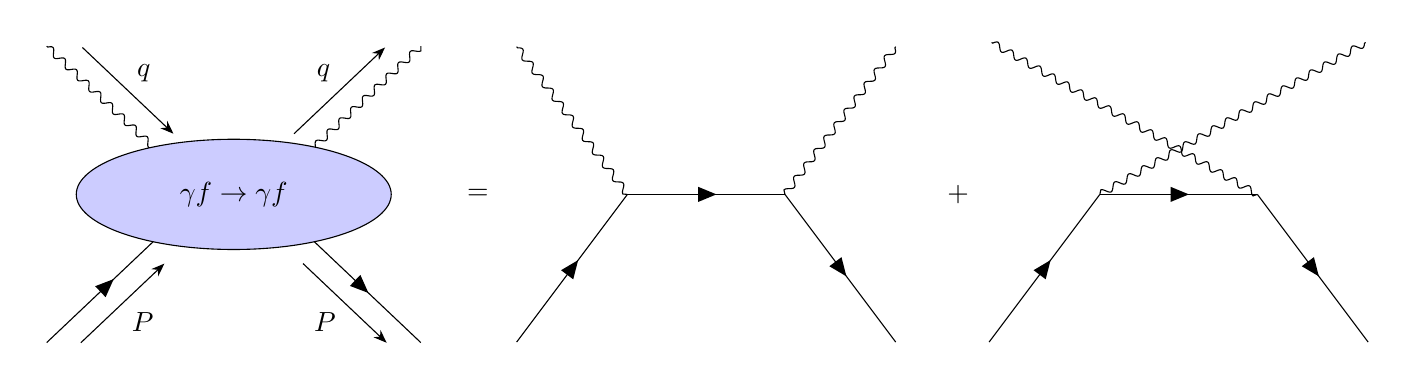
\begin{tikzpicture}
    \begin{feynman}
        %% 顶点
        \vertex (j0) at (0,0){j0};
        %%
        \vertex[above right =0.2  and -0.6 of j0] (h1){};
        \vertex[above right =0.2  and +0.6 of j0] (h2){};
        \vertex[above right =2  and 2.5 of j0] (j3){};
        \vertex[above right =2  and -2.5 of j0] (j4){};
        %%
        \vertex[above right =-0.2  and -0.6 of j0] (k1){k1};
        \vertex[above right =-0.2  and +0.6 of j0] (k2){k2};
        \vertex[above right =-2  and -2.5 of j0] (j1){};
        \vertex[above right =-2  and 2.5 of j0] (j2){};
        %% 图2
        \node[anchor=center] at (3.1,0){$=$};
        \vertex (x0) at (6,0){};
        %---
        \vertex[above right =-2 and -2.5 of x0] (x1){};
        \vertex[above right =-2 and +2.5 of x0] (x2){};
        \vertex[above right =0  and -1 of x0] (x5);
        \vertex[above right =0  and +1 of x0] (x6);
        %---
        \vertex[above right =2  and -2.5 of x0] (x3){};
        \vertex[above right =2  and +2.5 of x0] (x4){};
        %% 图3
        \node[anchor=center] at (9.2,0){$+$};
        \vertex (y0) at (12,0){};
        %---
        \vertex[above right =-2 and -2.5 of y0] (y1){};
        \vertex[above right =-2 and +2.5 of y0] (y2){};
        \vertex[above right =0  and -1 of y0] (y5);
        \vertex[above right =0  and +1 of y0] (y6);
        %---
        \vertex[above right =2  and -2.5 of y0] (y3){};
        \vertex[above right =2  and +2.5 of y0] (y4){};
        % 对各个顶点连线
        \diagram*{
        { [edge= fermion]
        (j1) --[momentum'=\(P\)] (k1)--(k2)--[momentum'=\(P\)](j2),
        (x1) --(x5)--(x6)--(x2),
        (y1) --(y5)--(y6)--(y2),
        };
        % 光子线
        {[edge=photon]
        (j4) --[momentum=\(q\)] (h1)--(h2)--[momentum=\(q\)](j3),
        (x3)--(x5),(x4)--(x6),
        (y3)--(y6),(y4)--(y5),
        };
        };
        % 画椭圆 blob
        \filldraw[fill=blue!20,draw=black] (j0)
        ellipse[x radius=2,y radius=0.7,anchor=center];
        % 文字
        \node[above right =0  and 0 of j0] (t1)
        {$\gamma f\to\gamma f$};
    \end{feynman}
\end{tikzpicture}
\end{document}